\documentclass[11pt,a4paper]{amsart}

\usepackage[margin=1in]{geometry}
\usepackage{graphicx}
\usepackage{amsmath}
\usepackage{amsfonts}
\usepackage{amsthm}
\usepackage{mathrsfs}
\usepackage{float}
\usepackage{subfig}
\usepackage{hyperref}
\usepackage{dsfont}



\newtheorem{thm}{Theorem}[section]
\newtheorem{ex}{Example}
\newtheorem{prb}{Problem}
\newtheorem{pf}{Proof}
\newtheorem{lem}[thm]{Lemma}
\newtheorem{prop}[thm]{Proposition}
\newtheorem{cor}[thm]{Corollary}
\newtheorem{conj}[thm]{Conjecture}
\newtheorem{defn}{Definition}[section]
\newtheorem{example}{Example}[section]

\newcommand{\PP}{\mathbb{P}}		%Used for probabilities.
\newcommand{\NN}{\mathbb{N}}		%Used to denote the natural numbers.
\newcommand{\RR}{\mathbb{R}}		%Used to denote the real numbers.
\newcommand{\statespace}{\mathscr{S}}	%Used to denote the state space.
\newcommand{\MM}{\mathscr{M}}		%Used to denote the space of measurable sets.
\newcommand{\CC}{\mathbb{C}}
\DeclareMathOperator{\Var}{\text{Var}}
\newcommand{\s}{\sigma}
\newcommand{\W}{\widetilde{W}}
\newcommand{\w}{\omega}
\newcommand{\EE}{\mathbb{E}}
\newcommand{\N}{\mathcal{N}}


\begin{document}
\title{Monte Carlo Methods: HW 3}
\author{Terrence Alsup}
\date{March 27th, 2019}
\maketitle

\emph{Note: The MCMC methods are implemented in the Python file {\tt IsingSamplers.py}}.

\vspace{0.5in}

%%%%%%%%%%%%%%%%%%%%%%%%%%%%%%%%%%%%%%

{\bf Exercise 39}\\
\\
\par The Python file {\tt IsingSamplers.py} contains a function called {\tt IsingSampler} which can be called with the option to use Gibbs sampling by repeatedly calling the function {\tt GibbsUpdate}, which is just a single step in the Markov chain.  Given a length $N$ of the chain we can obtain an approximate sample of the 2D Ising model with distribution
\[
\pi(\sigma) = \frac{1}{Z} \exp\left(  \beta \sum_{\vec{i} \leftrightarrow \vec{j}} \sigma_{\vec{i}}\ \sigma_{\vec{j}} \right)
\]
Here $\beta \propto T^{-1}$ is the inverse temperature and each $\vec{i} \in \mathbb{Z}_L^2$.  When $\beta > 0$ this is a model for ferromagnets.  The configurations with the highest probability are the ones where all spins $\sigma_{\vec{i}}$ are the same.  If $\beta < 0$, then this is a model for anti-ferromagnets, where the most likely configurations are the ones in which all of the spins are opposite of their neighbors (checkerboard pattern).  We can check how this model behaves for different $\beta$ by examining the magnetization of the lattice
\[
f(\sigma) = \sum_{\vec{i} \in \mathbb{Z}_L^2} \sigma_{\vec{i}}
\]
Figures~\ref{fig:maghistb1} and \ref{fig:maghistb005} below show histograms of the average magnetization (normalized between $-1$ and $1$) for two different values of $\beta$.  At $\beta \approx 0.44$ (see \cite{IsingWiki}) there is a phase transition where spontaneous magnetization can occur.  If the temperature is low enough, meaning $\beta \gg 0.44$, then eventually all spins will become aligned with very high probability as shown in Figure~\ref{fig:maghistb1}.  On the other hand, for sub-critical $\beta$, meaning high temperatures, the spins are almost independent.  In this regime, by the central limit theorem, the magnetization has approximately a Gaussian distribution which is shown in Figure~\ref{fig:maghistb005}.



\begin{figure}[H]
\centering
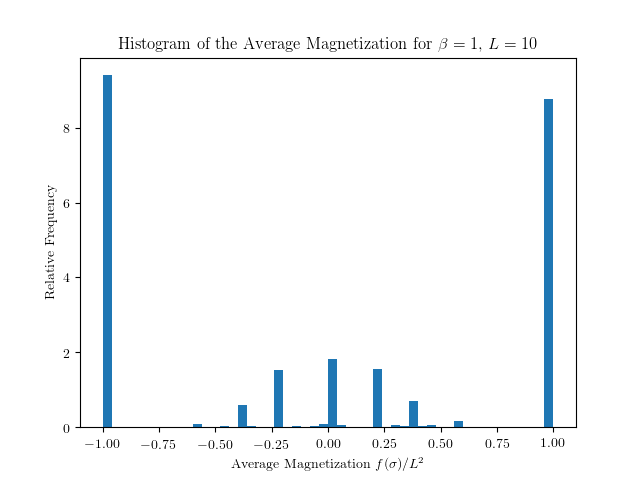
\includegraphics[width=5in]{maghistb1.png}
\caption{A histogram of 1000 samples of the average magnetization from the 2D Ising Model.  Gibbs sampling was used with the length of each chain being 10000 steps.  The lattice site to update at each step was chosen randomly.}
\label{fig:maghistb1}
\end{figure}

\begin{figure}[H]
\centering
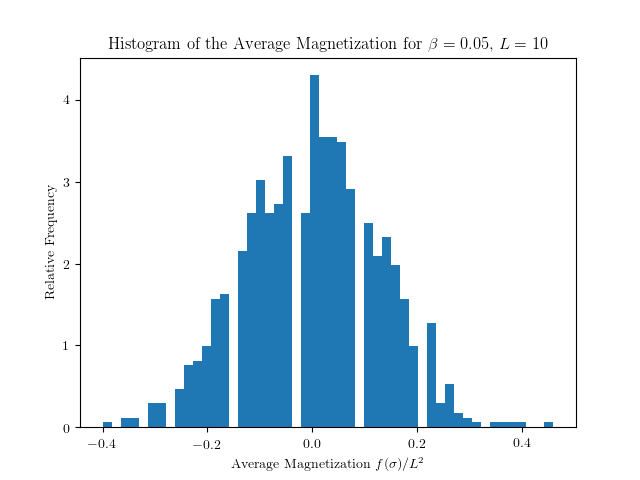
\includegraphics[width=5in]{maghistb005.png}
\caption{A histogram of 1000 samples of the average magnetization from the 2D Ising Model.  Gibbs sampling was used with the length of each chain being 10000 steps.  The lattice site to update at each step was chosen randomly.}
\label{fig:maghistb005}
\end{figure}


\par To determine how good our sampler is we can estimate the integrated autocorrelation time $\tau$ of the magnetization. To estimate $\tau$ we use the Python package {\tt acor}.  Figure~\ref{fig:gibbsRandomACFb005} below shows the autocorrelation function of the magnetization.  We see that when $L = 10$ and $\beta = 0.05$ it takes $\approx 700$ Gibbs steps for the correlation to decay to 0.  Because after this point the noise dominates our estimate, we truncate our calculation of the integrated autocorrelation time
\[
\hat{\tau} = 1+ 2\sum_{k=1}^{700}\text{corr}_{\pi}(f(X^{(0)}),\  f(X^{(k)}))
\]
We compute $\hat{\tau}$ for chains of length $10^{5},10^6$, and $10^7$ to see that it converges to $\tau \approx 320$.  By the same procedure, we estimate that $\hat{\tau} \approx 165$ if we instead sweep through the sites left-to-right and top-to-bottom deterministically, which is much better.  In particular, it means our effective sample size is twice as large for a fixed chain length whenever we sweep through deterministically.

\begin{figure}[H]
\centering
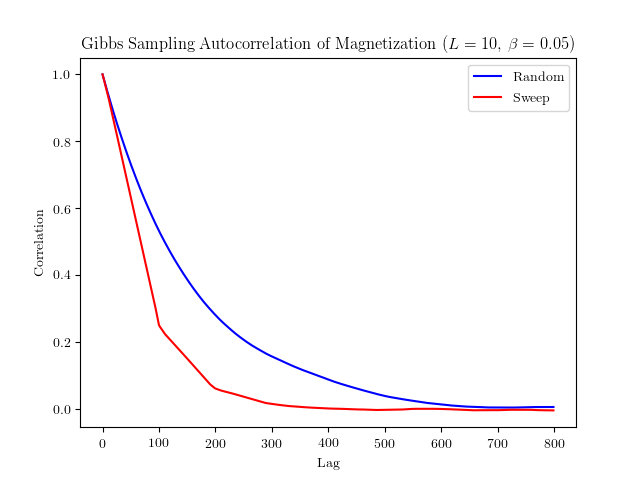
\includegraphics[width=5in]{gibbsRandomACFb005.png}
\caption{The estimated autocorrelation function of the magnetization using Gibbs sampling.  The length of the chain was $10^6$, but we truncate for a maximum lag of 800, after which point the noise begins to accumulate.  The correlation for a deterministic sweep decays much faster.}
\label{fig:gibbsRandomACFb005}
\end{figure}




%%%%%%%%%%%%%%%%%%%%%%%%%%%%%%%%%%%%%%

{\bf Exercise 42}\\
\\
\par The estimated IAC for Metropolis-Hastings was $\hat{\tau} \approx 189$ by running chains of length $10^5, 10^6$, and $10^7$.  The proposal distribution at each step was to randomly select a site and change its sign with probability.

\begin{figure}[H]
\centering
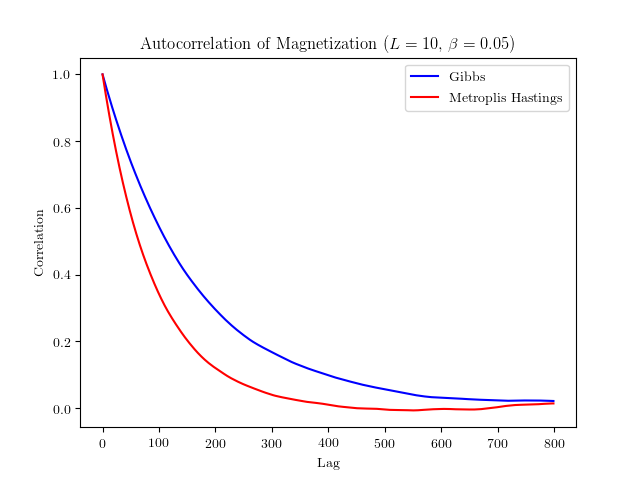
\includegraphics[width=5in]{gibbsMHACF.png}
\caption{The estimated autocorrelation function of the magnetization using Gibbs sampling.  The length of the chain was $10^6$, but we truncate for a maximum lag of 800, after which point the noise begins to accumulate.  The correlation for Metropolis-Hastings decays faster.}
\label{fig:gibbsRandomACFb005}
\end{figure}

%%%%%%%%%%%%%%%%%%%%%%%%%%%%%%%%%%%%%%

\begin{thebibliography}{10}

\bibitem{IsingWiki}
Square-lattice Ising Model.\\
\texttt{https://en.wikipedia.org/wiki/Square-lattice\_Ising\_model}

\vspace{0.1in}

\bibitem{Liu}
Jun Liu (2004). \emph{Monte Carlo Strategies in Scientific Computing}.

\end{thebibliography}

%%%%%%%%%%%%%%%%%%%%%%%%%%%%%%%%%%%%%%

\end{document}
